% Options for packages loaded elsewhere
\PassOptionsToPackage{unicode}{hyperref}
\PassOptionsToPackage{hyphens}{url}
%
\documentclass[
]{article}
\usepackage{amsmath,amssymb}
\usepackage{iftex}
\ifPDFTeX
  \usepackage[T1]{fontenc}
  \usepackage[utf8]{inputenc}
  \usepackage{textcomp} % provide euro and other symbols
\else % if luatex or xetex
  \usepackage{unicode-math} % this also loads fontspec
  \defaultfontfeatures{Scale=MatchLowercase}
  \defaultfontfeatures[\rmfamily]{Ligatures=TeX,Scale=1}
\fi
\usepackage{lmodern}
\ifPDFTeX\else
  % xetex/luatex font selection
\fi
% Use upquote if available, for straight quotes in verbatim environments
\IfFileExists{upquote.sty}{\usepackage{upquote}}{}
\IfFileExists{microtype.sty}{% use microtype if available
  \usepackage[]{microtype}
  \UseMicrotypeSet[protrusion]{basicmath} % disable protrusion for tt fonts
}{}
\makeatletter
\@ifundefined{KOMAClassName}{% if non-KOMA class
  \IfFileExists{parskip.sty}{%
    \usepackage{parskip}
  }{% else
    \setlength{\parindent}{0pt}
    \setlength{\parskip}{6pt plus 2pt minus 1pt}}
}{% if KOMA class
  \KOMAoptions{parskip=half}}
\makeatother
\usepackage{xcolor}
\usepackage[margin=1in]{geometry}
\usepackage{longtable,booktabs,array}
\usepackage{calc} % for calculating minipage widths
% Correct order of tables after \paragraph or \subparagraph
\usepackage{etoolbox}
\makeatletter
\patchcmd\longtable{\par}{\if@noskipsec\mbox{}\fi\par}{}{}
\makeatother
% Allow footnotes in longtable head/foot
\IfFileExists{footnotehyper.sty}{\usepackage{footnotehyper}}{\usepackage{footnote}}
\makesavenoteenv{longtable}
\usepackage{graphicx}
\makeatletter
\def\maxwidth{\ifdim\Gin@nat@width>\linewidth\linewidth\else\Gin@nat@width\fi}
\def\maxheight{\ifdim\Gin@nat@height>\textheight\textheight\else\Gin@nat@height\fi}
\makeatother
% Scale images if necessary, so that they will not overflow the page
% margins by default, and it is still possible to overwrite the defaults
% using explicit options in \includegraphics[width, height, ...]{}
\setkeys{Gin}{width=\maxwidth,height=\maxheight,keepaspectratio}
% Set default figure placement to htbp
\makeatletter
\def\fps@figure{htbp}
\makeatother
\setlength{\emergencystretch}{3em} % prevent overfull lines
\providecommand{\tightlist}{%
  \setlength{\itemsep}{0pt}\setlength{\parskip}{0pt}}
\setcounter{secnumdepth}{5}
\ifLuaTeX
\usepackage[bidi=basic]{babel}
\else
\usepackage[bidi=default]{babel}
\fi
\babelprovide[main,import]{spanish}
% get rid of language-specific shorthands (see #6817):
\let\LanguageShortHands\languageshorthands
\def\languageshorthands#1{}
\usepackage[spanish]{babel}
\addto\captionsspanish{\renewcommand{\tablename}{Tabla}}
\addto\captionsspanish{\renewcommand{\listtablename}{Índice de tablas}}
\ifLuaTeX
  \usepackage{selnolig}  % disable illegal ligatures
\fi
\usepackage{bookmark}
\IfFileExists{xurl.sty}{\usepackage{xurl}}{} % add URL line breaks if available
\urlstyle{same}
\hypersetup{
  pdftitle={Informe Estandarización Perú Escala DINI},
  pdfauthor={Martín Vargas Estrada},
  pdflang={es},
  hidelinks,
  pdfcreator={LaTeX via pandoc}}

\title{Informe Estandarización Perú Escala DINI}
\author{Martín Vargas Estrada}
\date{2024-12-24 10:20:43.54687}

\begin{document}
\maketitle

{
\setcounter{tocdepth}{2}
\tableofcontents
}
\listoftables
\newpage

\section{Introducción}\label{introducciuxf3n}

Informe de Exploración Psicométrica de los puntajes de la prueba DINI obtenidas con muestra de Perú, grupos Nivel 3, y Niveles 4-5 años.

\section{Análisis Descriptivo Nivel 3}\label{anuxe1lisis-descriptivo-nivel-3}

Pasaremos a describir y graficar las principales variables demográficas que caracterizan a la muestra:

\begin{enumerate}
\def\labelenumi{\arabic{enumi}.}
\tightlist
\item
  Fecha de Inicio
\item
  Edad en meses
\item
  Cuatrimestre de nacimiento
\item
  Grupo de Codmod
\item
  Región Natural
\item
  Área
\item
  Nivel Modalidad
\item
  Gestión
\item
  Departamento
\item
  Distrito
\item
  Quintil de Pobreza
\item
  Incidencia / No Incidencia (VSS)
\item
  Incidencia Perinatal
\item
  Inc.~Tratamiento Médico
\item
  Inc.~Patología
\item
  Inc.~Negligencia
\item
  Inc.~Mudanza
\item
  Inc.~Consumo
\item
  Inc.~Desempleo
\item
  Inc.~Familiar
\item
  Inc.~Otros
\item
  Tratamiento Técnico
\item
  Tratamiento Psicológico
\item
  Tratamiento Psiquiátrico
\item
  Tratamiento Pedagógico
\item
  Tratamiento Psicomotriz
\item
  Tratamiento Fonoaudiológico
\item
  Tratamiento Dificultades Diagnosticadas
\item
  Tratamiento Discapacidad
\item
  Tratamiento Ninguno
\item
  Instrucción Previa al Nivel 3
\item
  Nivel
\end{enumerate}

\subsection{Fechas de Evaluación}\label{fechas-de-evaluaciuxf3n}

A continuación veamos la distribución según las fechas de evaluación:

\begin{table}

\caption{(\#tab:30_Dem_FechAp)Frecuencias de Fechin}
\centering
\begin{tabular}[t]{lrrrr}
\toprule
Fechin & N & \% & N Acum. & \% Acum.\\
\midrule
04/29/2024 & 270 & 24.88 & 270 & 24.88\\
05/20/2024 & 225 & 20.74 & 495 & 45.62\\
06/17/2024 & 305 & 28.11 & 800 & 73.73\\
08/12/2024 & 285 & 26.27 & 1085 & 100.00\\
\bottomrule
\end{tabular}
\end{table}

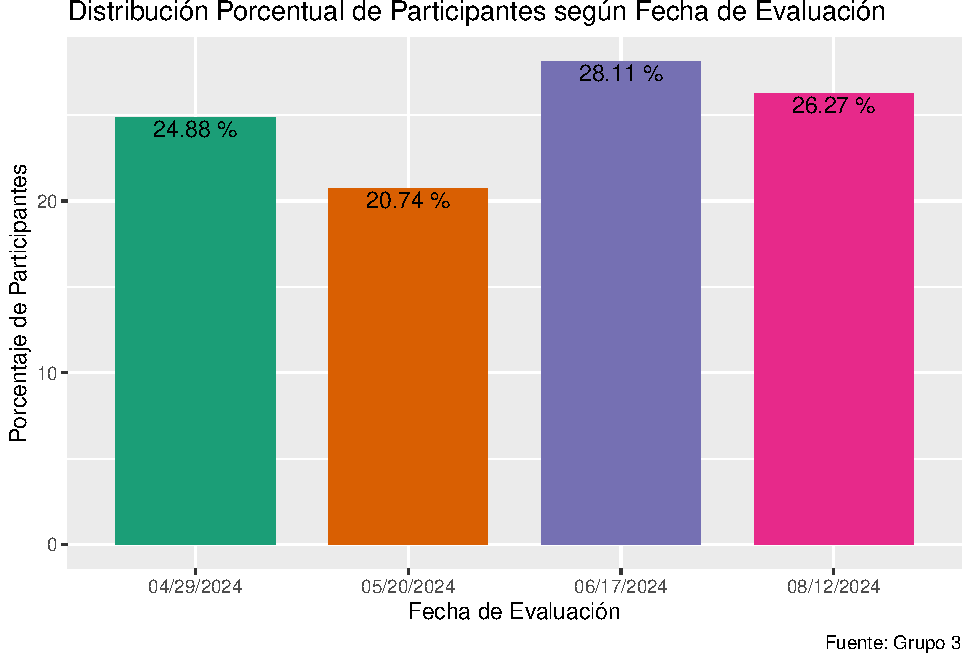
\includegraphics{CopyOfInfo_Dinix_02-beta_files/figure-latex/30_Dem_FechAp-1.pdf}

\subsection{Edad en Meses}\label{edad-en-meses}

A continuación, la información acerca de la edad en meses del participante

\begin{table}

\caption{(\#tab:30_Dem_Age_Mo)Frecuencias de EDADMES}
\centering
\begin{tabular}[t]{lrrrr}
\toprule
EDADMES & N & \% & N Acum. & \% Acum.\\
\midrule
32 & 1 & 0.09 & 1 & 0.09\\
33 & 1 & 0.09 & 2 & 0.18\\
36 & 5 & 0.46 & 7 & 0.64\\
37 & 14 & 1.29 & 21 & 1.93\\
38 & 33 & 3.04 & 54 & 4.97\\
\addlinespace
39 & 51 & 4.70 & 105 & 9.67\\
40 & 58 & 5.35 & 163 & 15.02\\
41 & 80 & 7.37 & 243 & 22.39\\
42 & 79 & 7.28 & 322 & 29.67\\
43 & 70 & 6.45 & 392 & 36.12\\
\addlinespace
44 & 74 & 6.82 & 466 & 42.94\\
45 & 78 & 7.19 & 544 & 50.13\\
46 & 91 & 8.39 & 635 & 58.52\\
47 & 89 & 8.20 & 724 & 66.72\\
48 & 97 & 8.94 & 821 & 75.66\\
\addlinespace
49 & 93 & 8.57 & 914 & 84.23\\
50 & 62 & 5.71 & 976 & 89.94\\
51 & 31 & 2.86 & 1007 & 92.80\\
52 & 20 & 1.84 & 1027 & 94.64\\
53 & 7 & 0.65 & 1034 & 95.29\\
\addlinespace
54 & 5 & 0.46 & 1039 & 95.75\\
55 & 10 & 0.92 & 1049 & 96.67\\
56 & 3 & 0.28 & 1052 & 96.95\\
57 & 4 & 0.37 & 1056 & 97.32\\
59 & 5 & 0.46 & 1061 & 97.78\\
\addlinespace
60 & 3 & 0.28 & 1064 & 98.06\\
61 & 5 & 0.46 & 1069 & 98.52\\
62 & 6 & 0.55 & 1075 & 99.07\\
63 & 7 & 0.65 & 1082 & 99.72\\
64 & 3 & 0.28 & 1085 & 100.00\\
\bottomrule
\end{tabular}
\end{table}

\begin{longtable}[]{@{}lrrrr@{}}
\toprule\noalign{}
Variable & Mediana & Media & Desviación.Estándar & Número.de.Casos \\
\midrule\noalign{}
\endhead
\bottomrule\noalign{}
\endlastfoot
EDADMES & 45 & 45.51 & 4.88 & 1085 \\
\end{longtable}

A continuación el histograma de la Edad en meses:

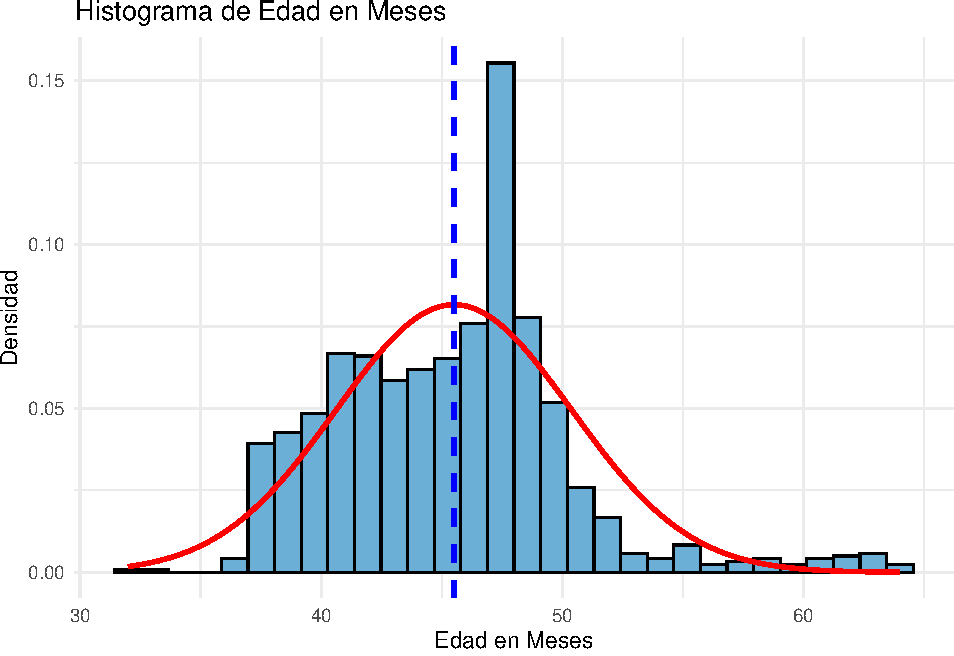
\includegraphics{CopyOfInfo_Dinix_02-beta_files/figure-latex/30_AgeMo_Hist-1.pdf}

\subsection{Cuatrimestre de Nacimiento}\label{cuatrimestre-de-nacimiento}

A continuación, la información acerca de la edad en meses del participante. Esta variable fue creada a partir de los datos de fecha de nacimiento de los participantes. El propósito es llegar a establecer, posteriormente, si existe relación entre el cuatrimestre de nacimiento del participante y el nivel de desempeño en la Escala DINI (relaciones similares han sido encontradas en estudios previos para otros instrumentos y mediciones de logro académico).

\begin{table}

\caption{(\#tab:30_QDOB)Frecuencias de QDOB}
\centering
\begin{tabular}[t]{lrrrr}
\toprule
QDOB & N & \% & N Acum. & \% Acum.\\
\midrule
1 (Ene-Mar) & 222 & 20.46 & 222 & 20.46\\
2 (Abr-Jun) & 342 & 31.52 & 564 & 51.98\\
3 (Jul-Sep) & 276 & 25.44 & 840 & 77.42\\
4 (Oct-Dic) & 245 & 22.58 & 1085 & 100.00\\
\bottomrule
\end{tabular}
\end{table}

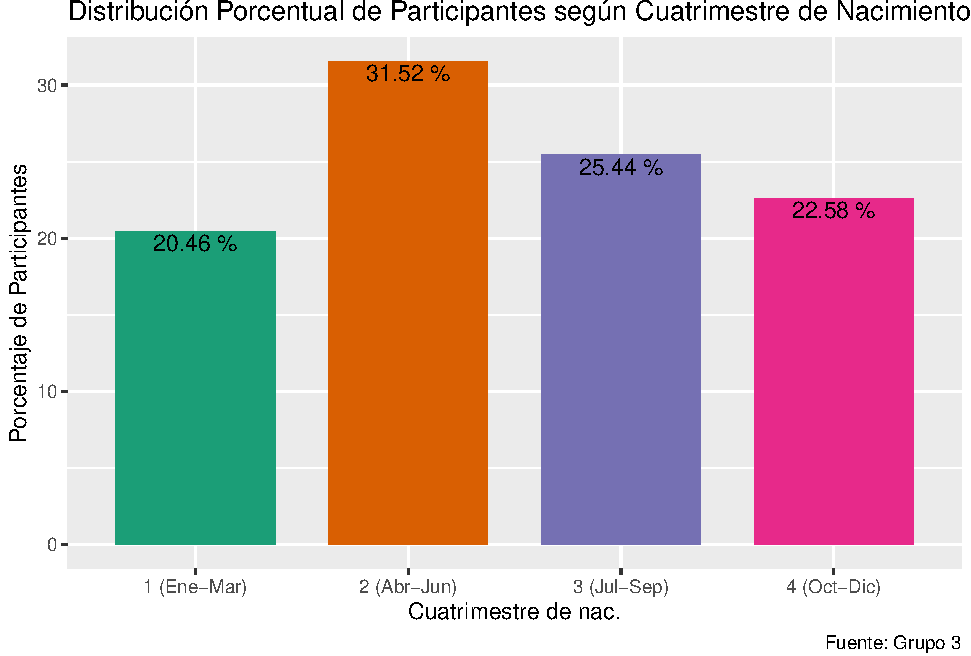
\includegraphics{CopyOfInfo_Dinix_02-beta_files/figure-latex/30_QDOB-1.pdf}

\subsection{Grupo CodMod}\label{grupo-codmod}

A continuación, la información acerca de CodMod

\begin{table}

\caption{(\#tab:30_CodMod)Frecuencias de Codmod}
\centering
\begin{tabular}[t]{lrrrr}
\toprule
Codmod & N & \% & N Acum. & \% Acum.\\
\midrule
0259432 & 52 & 4.79 & 52 & 4.79\\
0259630 & 39 & 3.59 & 91 & 8.38\\
0259648 & 39 & 3.59 & 130 & 11.97\\
0259770 & 21 & 1.94 & 151 & 13.91\\
0335422 & 75 & 6.91 & 226 & 20.82\\
\addlinespace
0403659 & 33 & 3.04 & 259 & 23.86\\
0403675 & 13 & 1.20 & 272 & 25.06\\
0403964 & 55 & 5.07 & 327 & 30.13\\
0404079 & 19 & 1.75 & 346 & 31.88\\
0500215 & 18 & 1.66 & 364 & 33.54\\
\addlinespace
0540062 & 11 & 1.01 & 375 & 34.55\\
0542175 & 31 & 2.86 & 406 & 37.41\\
0551192 & 25 & 2.30 & 431 & 39.71\\
0565598 & 40 & 3.69 & 471 & 43.40\\
0565606 & 2 & 0.18 & 473 & 43.58\\
\addlinespace
0565952 & 23 & 2.12 & 496 & 45.70\\
0572446 & 1 & 0.09 & 497 & 45.79\\
0613646 & 39 & 3.59 & 536 & 49.38\\
0651901 & 15 & 1.38 & 551 & 50.76\\
0688838 & 18 & 1.66 & 569 & 52.42\\
\addlinespace
0730275 & 5 & 0.46 & 574 & 52.88\\
0750604 & 2 & 0.18 & 576 & 53.06\\
0772780 & 6 & 0.55 & 582 & 53.61\\
0774372 & 51 & 4.70 & 633 & 58.31\\
0838441 & 56 & 5.16 & 689 & 63.47\\
\addlinespace
0930842 & 15 & 1.38 & 704 & 64.85\\
1055763 & 24 & 2.21 & 728 & 67.06\\
1137579 & 18 & 1.66 & 746 & 68.72\\
1137942 & 9 & 0.83 & 755 & 69.55\\
1151570 & 5 & 0.46 & 760 & 70.01\\
\addlinespace
1152537 & 30 & 2.76 & 790 & 72.77\\
1188184 & 44 & 4.06 & 834 & 76.83\\
1262419 & 5 & 0.46 & 839 & 77.29\\
1262773 & 4 & 0.37 & 843 & 77.66\\
1321272 & 38 & 3.50 & 881 & 81.16\\
\addlinespace
1348036 & 4 & 0.37 & 885 & 81.53\\
1396605 & 3 & 0.28 & 888 & 81.81\\
1396647 & 14 & 1.29 & 902 & 83.10\\
1396720 & 3 & 0.28 & 905 & 83.38\\
1439017 & 2 & 0.18 & 907 & 83.56\\
\addlinespace
1440577 & 3 & 0.28 & 910 & 83.84\\
1440627 & 2 & 0.18 & 912 & 84.02\\
1491182 & 15 & 1.38 & 927 & 85.40\\
1504026 & 45 & 4.15 & 972 & 89.55\\
1516624 & 13 & 1.20 & 985 & 90.75\\
\addlinespace
1548437 & 7 & 0.65 & 992 & 91.40\\
1556232 & 10 & 0.92 & 1002 & 92.32\\
1559608 & 8 & 0.74 & 1010 & 93.06\\
1630029 & 32 & 2.95 & 1042 & 96.01\\
1674837 & 11 & 1.01 & 1053 & 97.02\\
\addlinespace
1714815 & 3 & 0.28 & 1056 & 97.30\\
1746148 & 11 & 1.01 & 1067 & 98.31\\
3013380 & 10 & 0.92 & 1077 & 99.23\\
3622240 & 8 & 0.74 & 1085 & 99.97\\
\bottomrule
\end{tabular}
\end{table}

\subsection{Región Natural}\label{regiuxf3n-natural}

A continuación, la información acerca de la Región Natural

\begin{table}

\caption{(\#tab:30_RegNat)Frecuencias de Regnat}
\centering
\begin{tabular}[t]{lrrrr}
\toprule
Regnat & N & \% & N Acum. & \% Acum.\\
\midrule
Costa & 489 & 45.07 & 489 & 45.07\\
Sierra & 277 & 25.53 & 766 & 70.60\\
Selva & 319 & 29.40 & 1085 & 100.00\\
\bottomrule
\end{tabular}
\end{table}

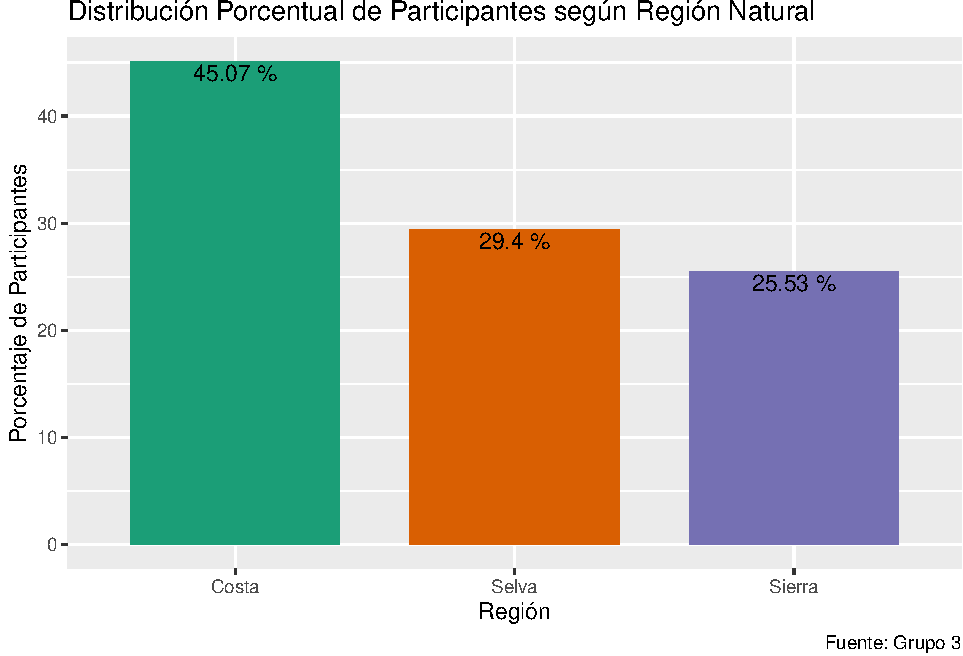
\includegraphics{CopyOfInfo_Dinix_02-beta_files/figure-latex/30_RegNat-1.pdf}

\subsection{Área}\label{uxe1rea}

A continuación, la información acerca del Área

\begin{table}

\caption{(\#tab:30_Area)Frecuencias de Area}
\centering
\begin{tabular}[t]{lrrrr}
\toprule
Area & N & \% & N Acum. & \% Acum.\\
\midrule
Urbana & 776 & 71.52 & 776 & 71.52\\
Rural & 309 & 28.48 & 1085 & 100.00\\
\bottomrule
\end{tabular}
\end{table}

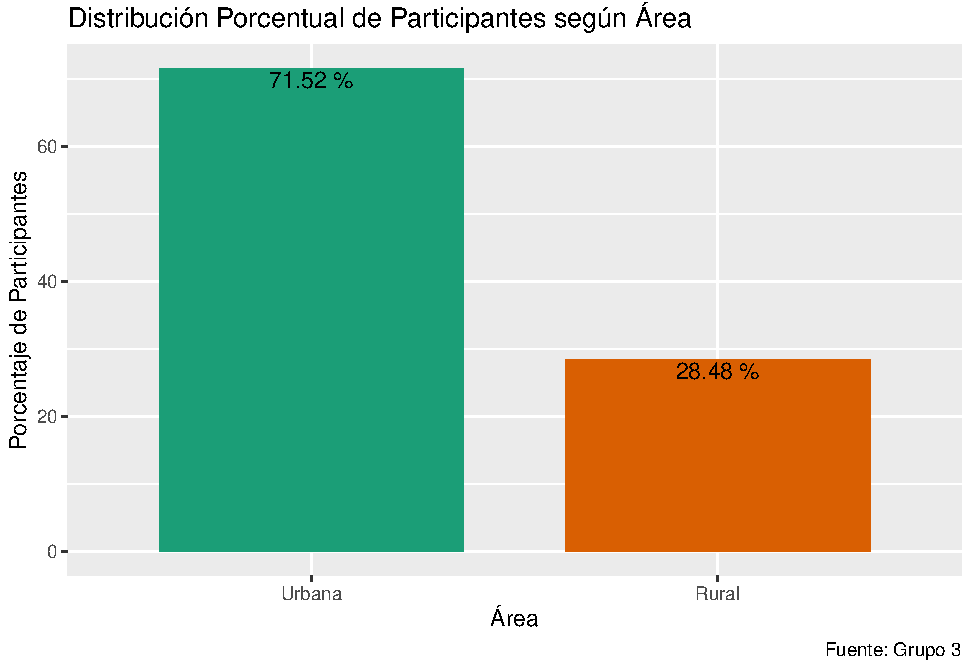
\includegraphics{CopyOfInfo_Dinix_02-beta_files/figure-latex/30_Area-1.pdf}

\subsection{Nivel de Modalidad}\label{nivel-de-modalidad}

A continuación, la información acerca del Nivel de Modalidad

\begin{table}

\caption{(\#tab:30_NivMod)Frecuencias de Nivmod}
\centering
\begin{tabular}[t]{lrrrr}
\toprule
Nivmod & N & \% & N Acum. & \% Acum.\\
\midrule
Inicial - Cuna-jardín & 184 & 16.96 & 184 & 16.96\\
Inicial - Jardín & 893 & 82.30 & 1077 & 99.26\\
Inicial - Programa no escolarizado & 8 & 0.74 & 1085 & 100.00\\
\bottomrule
\end{tabular}
\end{table}

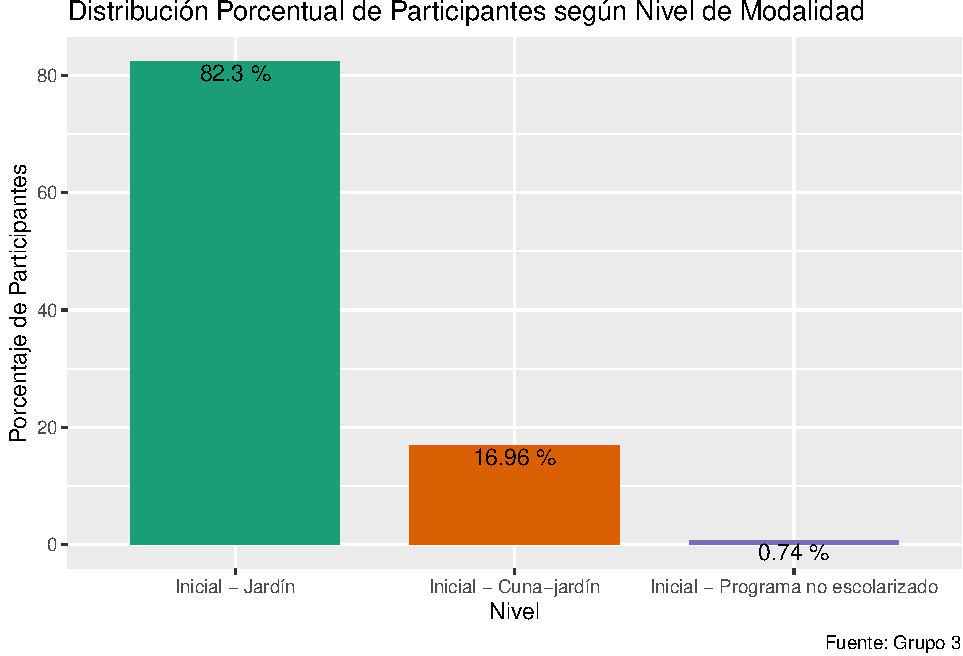
\includegraphics{CopyOfInfo_Dinix_02-beta_files/figure-latex/30_NivMod-1.pdf}

\subsection{Gestión}\label{gestiuxf3n}

A continuación, la información acerca de la Gestión (Pública o Privada) de la institución edicativa.

\begin{table}

\caption{(\#tab:30_Gest)Frecuencias de Gest}
\centering
\begin{tabular}[t]{lrrrr}
\toprule
Gest & N & \% & N Acum. & \% Acum.\\
\midrule
Pública & 967 & 89.12 & 967 & 89.12\\
Privada & 118 & 10.88 & 1085 & 100.00\\
\bottomrule
\end{tabular}
\end{table}

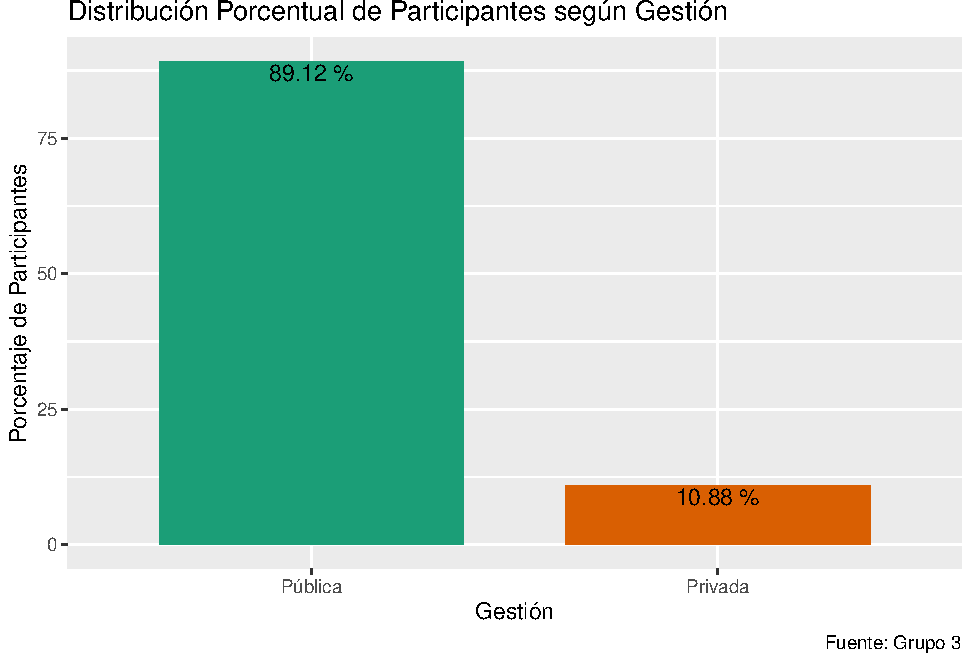
\includegraphics{CopyOfInfo_Dinix_02-beta_files/figure-latex/30_Gest-1.pdf}

\subsection{Departamento}\label{departamento}

A continuación, la información acerca del Departamento en donde vive el participante.

\begin{table}

\caption{(\#tab:30_Depa)Frecuencias de Reg}
\centering
\begin{tabular}[t]{lrrrr}
\toprule
Reg & N & \% & N Acum. & \% Acum.\\
\midrule
Cusco & 270 & 24.88 & 270 & 24.88\\
Lima Metropolitana & 285 & 26.27 & 555 & 51.15\\
Loreto & 225 & 20.74 & 780 & 71.89\\
Piura & 305 & 28.11 & 1085 & 100.00\\
\bottomrule
\end{tabular}
\end{table}

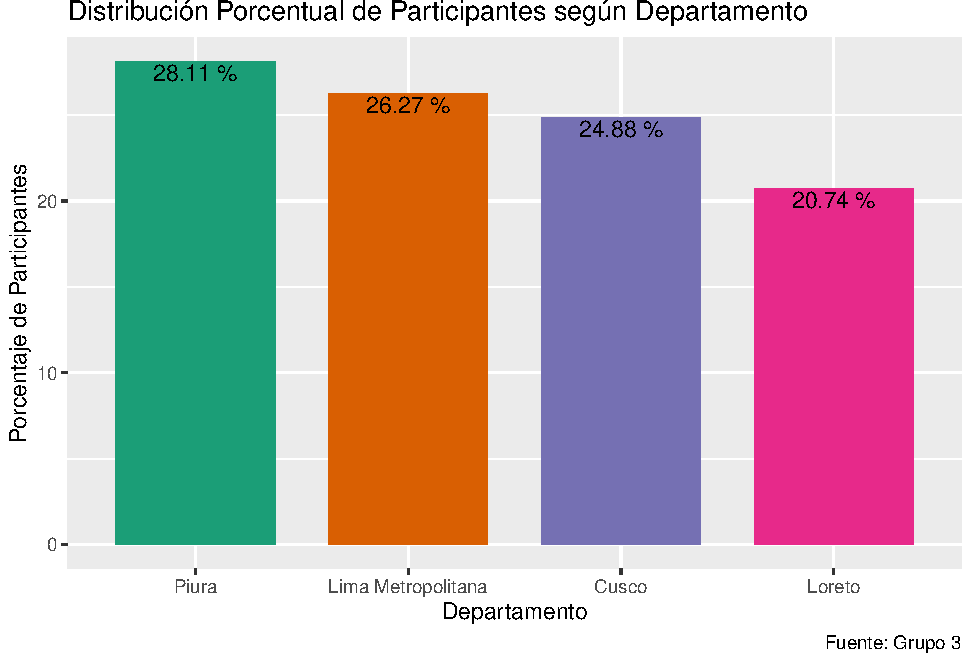
\includegraphics{CopyOfInfo_Dinix_02-beta_files/figure-latex/30_Depa-1.pdf}

\subsection{Quintil de Pobreza}\label{quintil-de-pobreza}

A continuación, la información acerca del Departamento en donde vive el participante.

\begin{table}

\caption{(\#tab:30_Quintus)Frecuencias de Quintil}
\centering
\begin{tabular}[t]{lrrrr}
\toprule
Quintil & N & \% & N Acum. & \% Acum.\\
\midrule
1 & 137 & 12.63 & 137 & 12.63\\
2 & 90 & 8.29 & 227 & 20.92\\
3 & 198 & 18.25 & 425 & 39.17\\
4 & 392 & 36.13 & 817 & 75.30\\
5 & 268 & 24.70 & 1085 & 100.00\\
\bottomrule
\end{tabular}
\end{table}

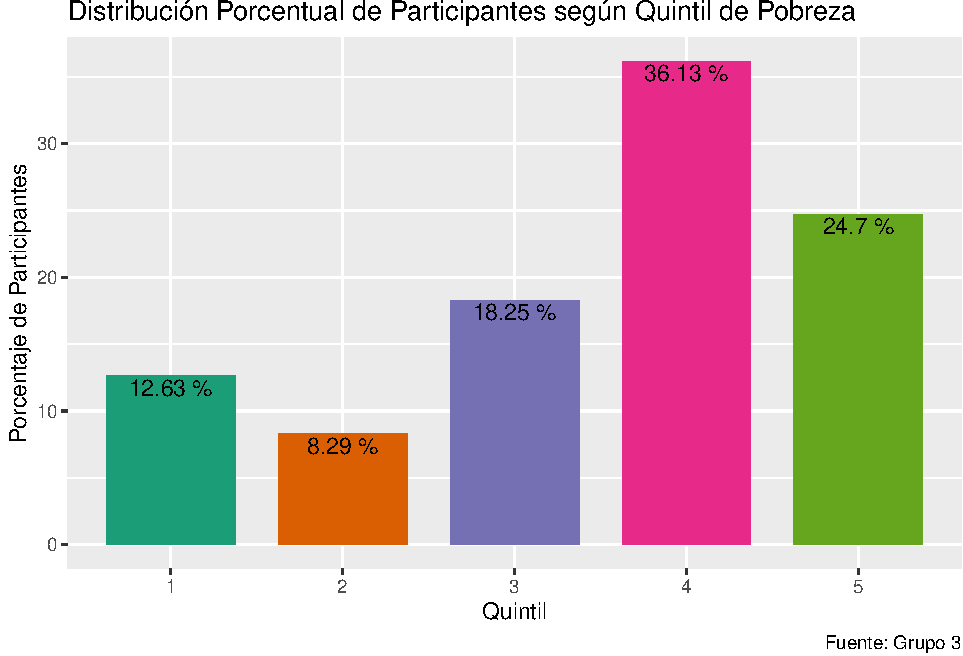
\includegraphics{CopyOfInfo_Dinix_02-beta_files/figure-latex/30_Quintus-1.pdf}

\subsection{Incidencia / No Incidencia (VSS)}\label{incidencia-no-incidencia-vss}

A continuación, la información acerca de la Incidencia / No Incidencia.

\begin{table}

\caption{(\#tab:30_VSS)Frecuencias de VSS}
\centering
\begin{tabular}[t]{lrrrr}
\toprule
VSS & N & \% & N Acum. & \% Acum.\\
\midrule
Ninguna & 976 & 89.95 & 976 & 89.95\\
Al Menos Una & 109 & 10.05 & 1085 & 100.00\\
\bottomrule
\end{tabular}
\end{table}

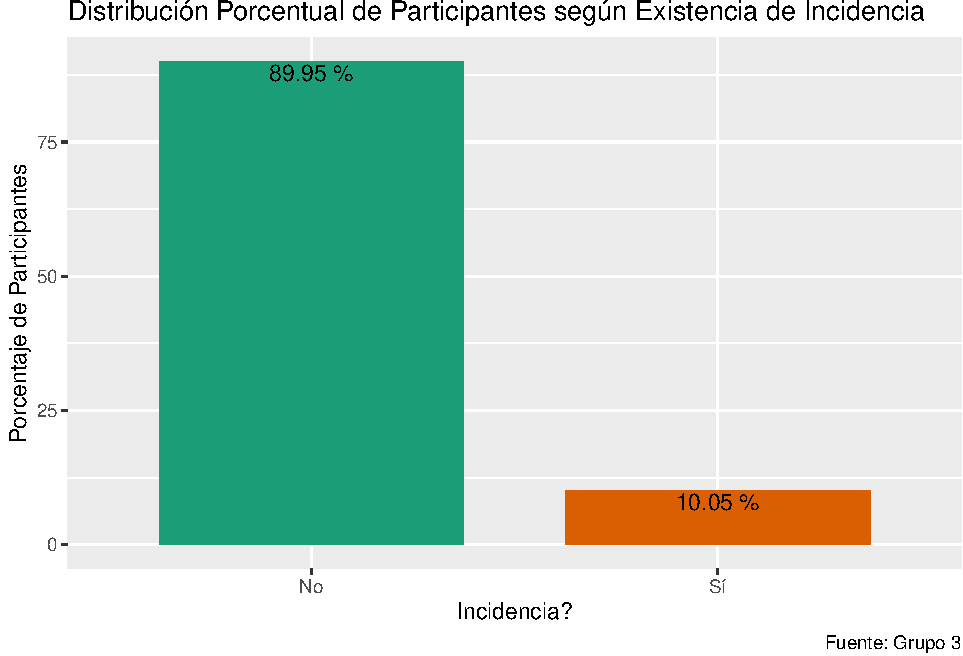
\includegraphics{CopyOfInfo_Dinix_02-beta_files/figure-latex/30_VSS-1.pdf}

\subsection{Incidencia Perinatal (VSSdesper)}\label{incidencia-perinatal-vssdesper}

A continuación, la información acerca de la Incidencia Perinatal.

\begin{table}

\caption{(\#tab:30_VSSdesper)Frecuencias de VSSdesper}
\centering
\begin{tabular}[t]{lrrrr}
\toprule
VSSdesper & N & \% & N Acum. & \% Acum.\\
\midrule
Ninguna & 1067 & 98.34 & 1067 & 98.34\\
Al Menos Una & 18 & 1.66 & 1085 & 100.00\\
\bottomrule
\end{tabular}
\end{table}

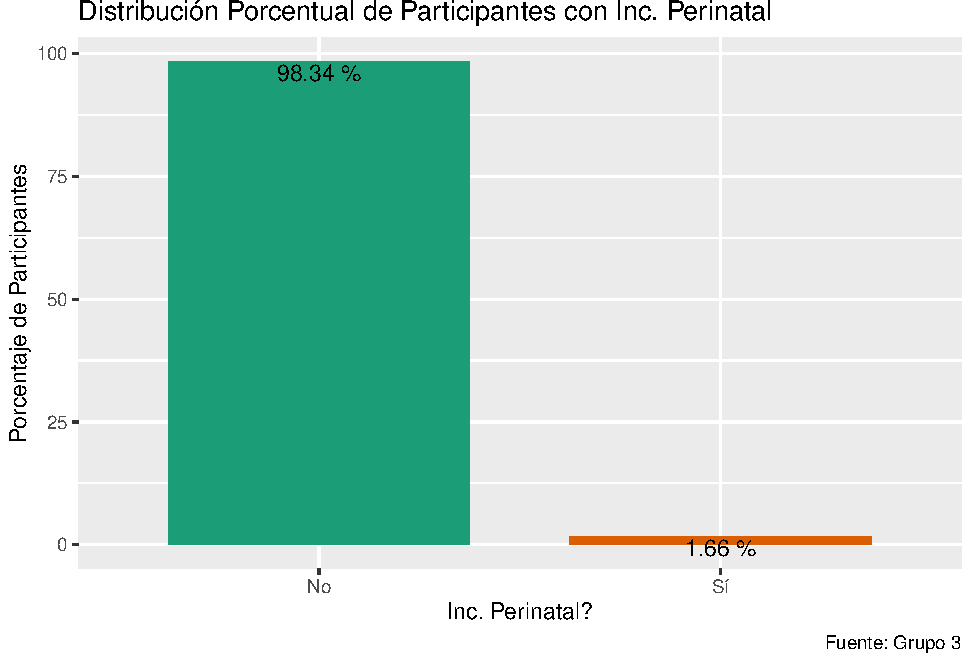
\includegraphics{CopyOfInfo_Dinix_02-beta_files/figure-latex/30_VSSdesper-1.pdf}

\subsection{Incidencia Tratamiento Médico (VSSttomed)}\label{incidencia-tratamiento-muxe9dico-vssttomed}

A continuación, la información acerca de la Incidencia por Tratamiento Médico.

\begin{table}

\caption{(\#tab:30_VSSttomed)Frecuencias de VSSttomed}
\centering
\begin{tabular}[t]{lrrrr}
\toprule
VSSttomed & N & \% & N Acum. & \% Acum.\\
\midrule
Ninguna & 1067 & 98.34 & 1067 & 98.34\\
Al Menos Una & 18 & 1.66 & 1085 & 100.00\\
\bottomrule
\end{tabular}
\end{table}

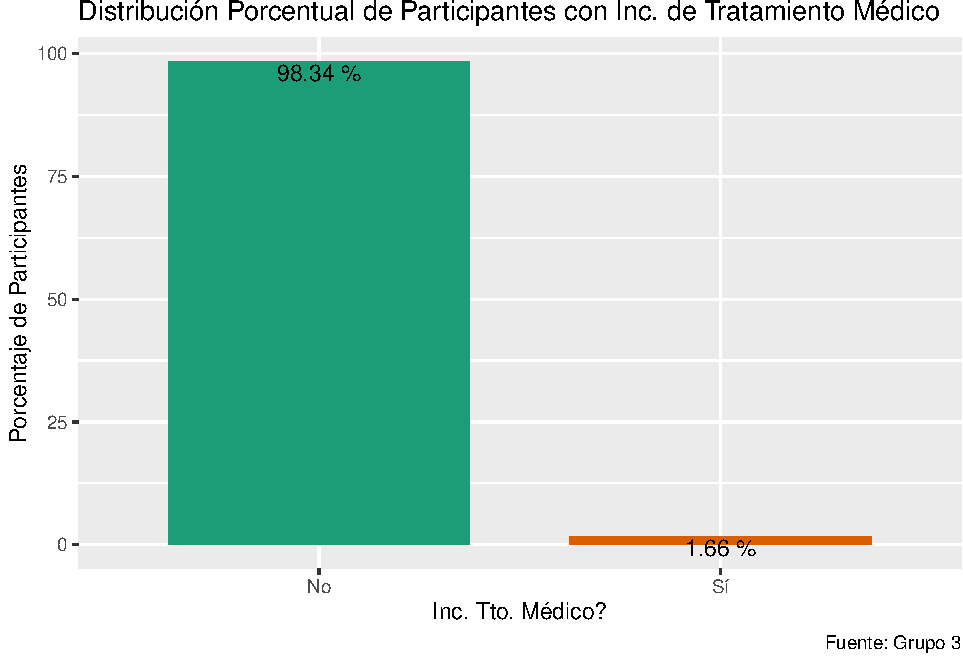
\includegraphics{CopyOfInfo_Dinix_02-beta_files/figure-latex/30_VSSttomed-1.pdf}

\subsection{Incidencia por Patología (VSSpatolo)}\label{incidencia-por-patologuxeda-vsspatolo}

A continuación, la información acerca de la Incidencia por Patología.

\begin{table}

\caption{(\#tab:30_VSSpatolo)Frecuencias de VSSpatolo}
\centering
\begin{tabular}[t]{lrrrr}
\toprule
VSSpatolo & N & \% & N Acum. & \% Acum.\\
\midrule
Ninguna & 1078 & 99.35 & 1078 & 99.35\\
Al Menos Una & 7 & 0.65 & 1085 & 100.00\\
\bottomrule
\end{tabular}
\end{table}

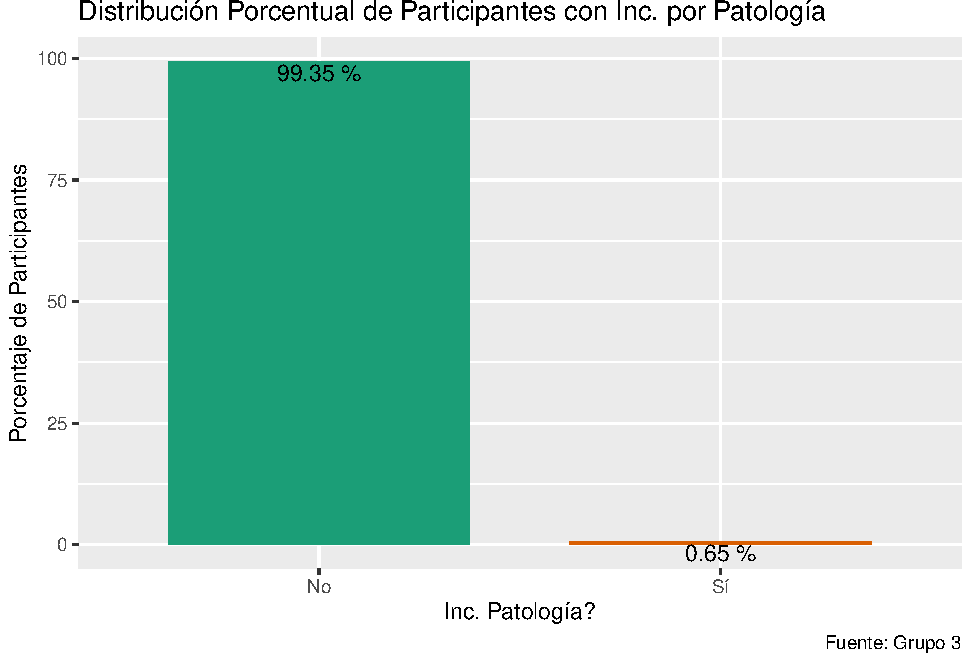
\includegraphics{CopyOfInfo_Dinix_02-beta_files/figure-latex/30_VSSpatolo-1.pdf}

\subsection{Incidencia por Negligencia (VSSnegl)}\label{incidencia-por-negligencia-vssnegl}

A continuación, la información acerca de la Incidencia por Negligencia

\begin{table}

\caption{(\#tab:30_VSSnegl)Frecuencias de VSSnegl}
\centering
\begin{tabular}[t]{lrrrr}
\toprule
VSSnegl & N & \% & N Acum. & \% Acum.\\
\midrule
Ninguna & 1080 & 99.54 & 1080 & 99.54\\
Al Menos Una & 5 & 0.46 & 1085 & 100.00\\
\bottomrule
\end{tabular}
\end{table}

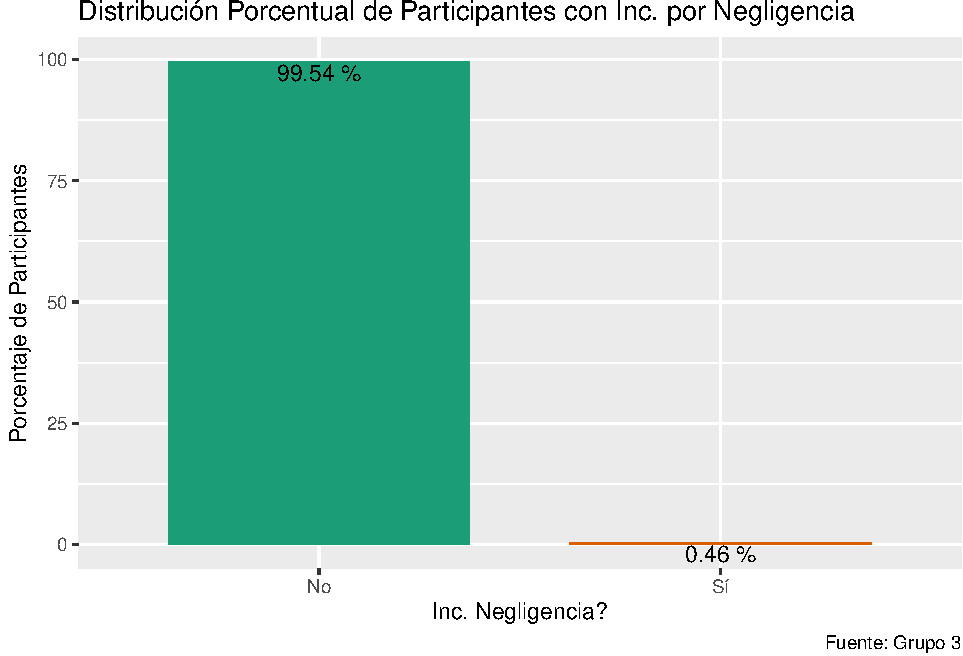
\includegraphics{CopyOfInfo_Dinix_02-beta_files/figure-latex/30_VSSnegl-1.pdf}

\subsection{Incidencia por Mudanza (VSSmud)}\label{incidencia-por-mudanza-vssmud}

A continuación, la información acerca de la Incidencia por Mudanza

\begin{table}

\caption{(\#tab:30_VSSmud)Frecuencias de VSSmud}
\centering
\begin{tabular}[t]{lrrrr}
\toprule
VSSmud & N & \% & N Acum. & \% Acum.\\
\midrule
Ninguna & 1055 & 97.24 & 1055 & 97.24\\
Al Menos Una & 30 & 2.76 & 1085 & 100.00\\
\bottomrule
\end{tabular}
\end{table}

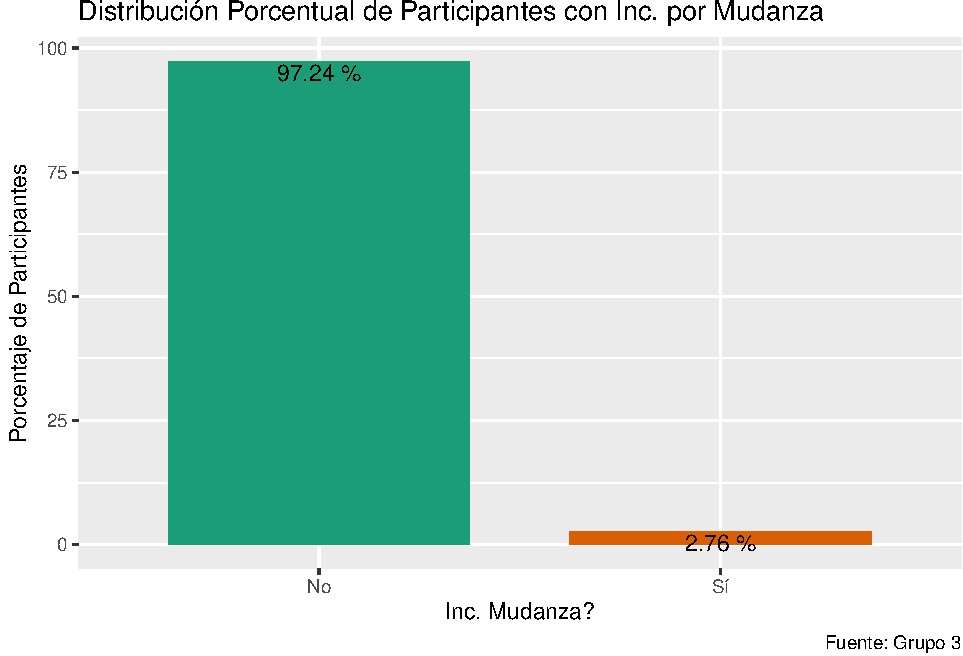
\includegraphics{CopyOfInfo_Dinix_02-beta_files/figure-latex/30_VSSmud-1.pdf}

\subsection{Incidencia por Consumo (VSSconsus)}\label{incidencia-por-consumo-vssconsus}

A continuación, la información acerca de la Incidencia por Consumo:

\begin{table}

\caption{(\#tab:30_VSSconsus)Frecuencias de VSSconsus}
\centering
\begin{tabular}[t]{lrrrr}
\toprule
VSSconsus & N & \% & N Acum. & \% Acum.\\
\midrule
Ninguna & 1080 & 99.54 & 1080 & 99.54\\
Al Menos Una & 5 & 0.46 & 1085 & 100.00\\
\bottomrule
\end{tabular}
\end{table}

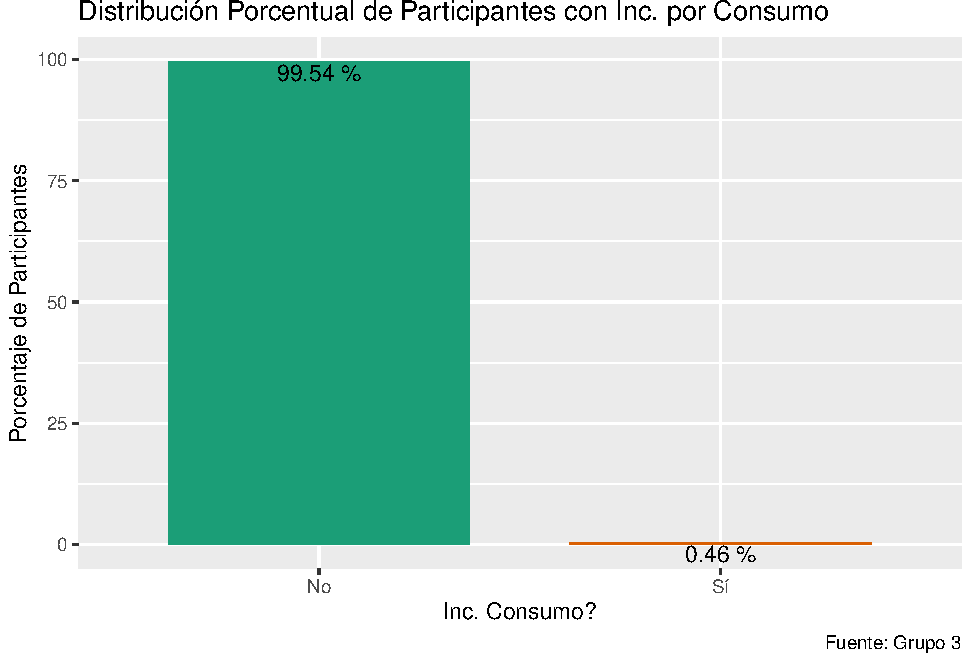
\includegraphics{CopyOfInfo_Dinix_02-beta_files/figure-latex/30_VSSconsus-1.pdf}

\subsection{Incidencia por Desempleo (VSSdesemp)}\label{incidencia-por-desempleo-vssdesemp}

A continuación, la información acerca de la Incidencia por Desempleo:

\begin{table}

\caption{(\#tab:30_VSSdesemp)Frecuencias de VSSdesemp}
\centering
\begin{tabular}[t]{lrrrr}
\toprule
VSSdesemp & N & \% & N Acum. & \% Acum.\\
\midrule
Ninguna & 1061 & 97.79 & 1061 & 97.79\\
Al Menos Una & 24 & 2.21 & 1085 & 100.00\\
\bottomrule
\end{tabular}
\end{table}

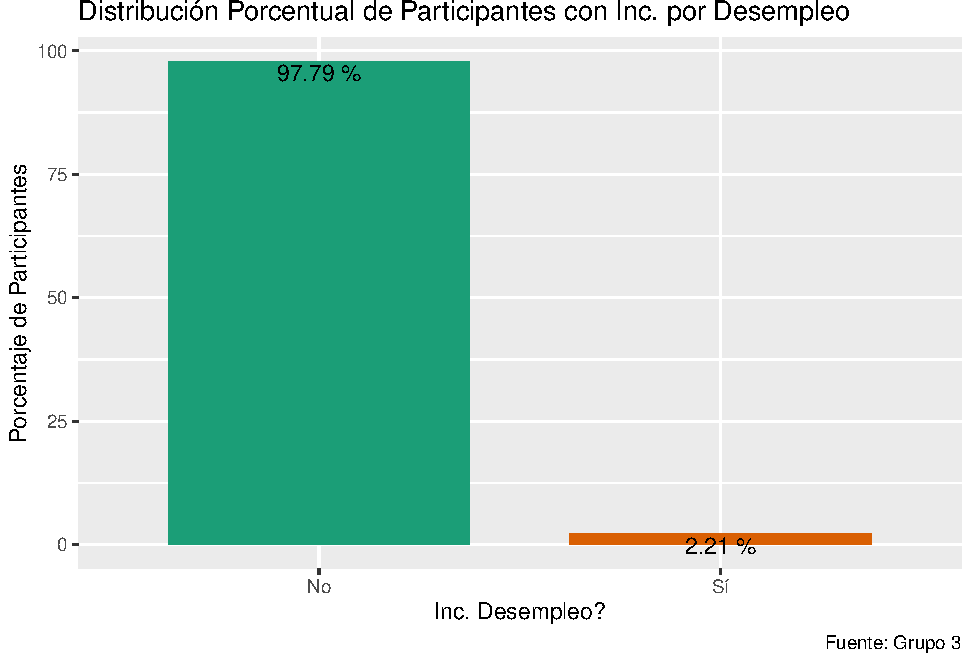
\includegraphics{CopyOfInfo_Dinix_02-beta_files/figure-latex/30_VSSdesemp-1.pdf}

\subsection{Incidencia Familiar (VSSfamprilib)}\label{incidencia-familiar-vssfamprilib}

A continuación, la información acerca de la Incidencia Familiar:

\begin{table}

\caption{(\#tab:30_VSSfamprilib)Frecuencias de VSSfamprilib}
\centering
\begin{tabular}[t]{lrrrr}
\toprule
VSSfamprilib & N & \% & N Acum. & \% Acum.\\
\midrule
Ninguna & 1084 & 99.91 & 1084 & 99.91\\
Al Menos Una & 1 & 0.09 & 1085 & 100.00\\
\bottomrule
\end{tabular}
\end{table}

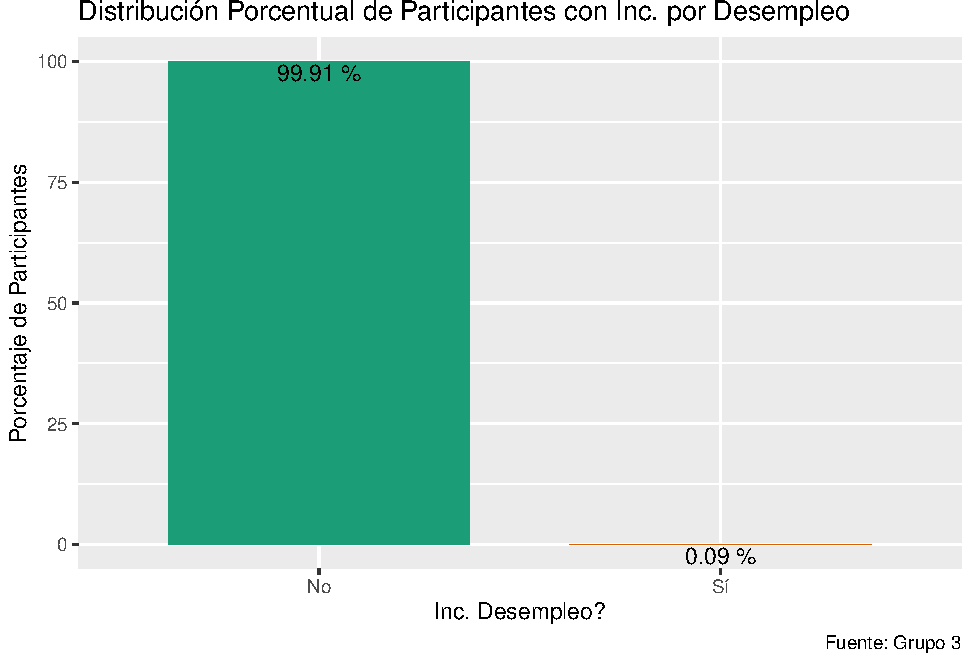
\includegraphics{CopyOfInfo_Dinix_02-beta_files/figure-latex/30_VSSfamprilib-1.pdf}

\subsection{Incidencia Otros (VSSotro)}\label{incidencia-otros-vssotro}

A continuación, la información acerca de la Incidencia Otros:

\begin{table}

\caption{(\#tab:30_VSSotro)Frecuencias de VSSotro}
\centering
\begin{tabular}[t]{lrrrr}
\toprule
VSSotro & N & \% & N Acum. & \% Acum.\\
\midrule
Ninguna & 1033 & 95.21 & 1033 & 95.21\\
Al Menos Una & 52 & 4.79 & 1085 & 100.00\\
\bottomrule
\end{tabular}
\end{table}

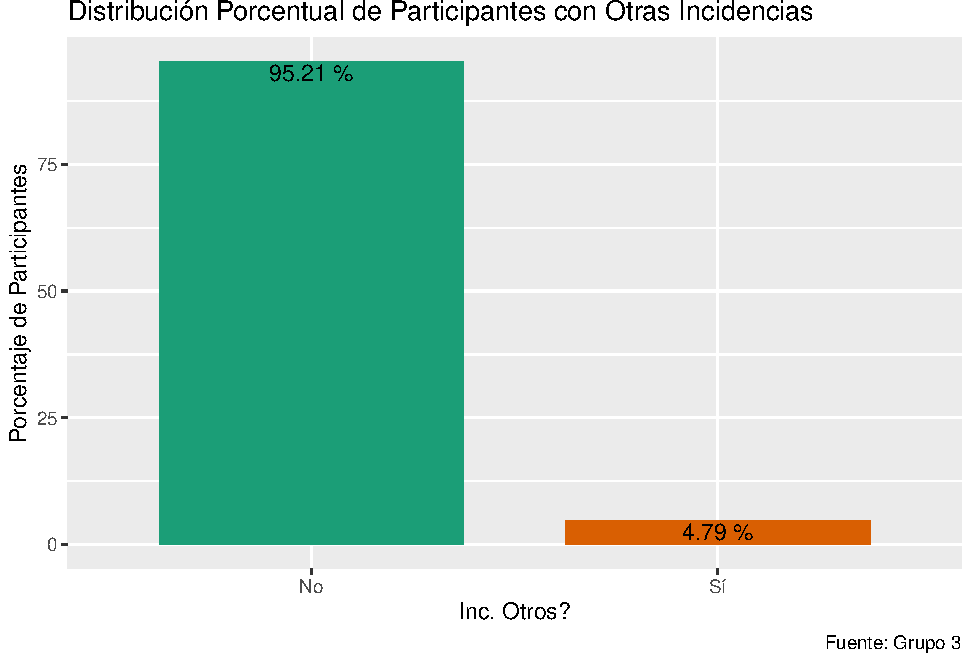
\includegraphics{CopyOfInfo_Dinix_02-beta_files/figure-latex/30_VSSotro-1.pdf}

\end{document}
